% Created 2020-12-08 Tue 17:19
% Intended LaTeX compiler: pdflatex
\documentclass{article}
\usepackage[utf8]{inputenc}
\usepackage[T1]{fontenc}
\usepackage{graphicx}
\usepackage{grffile}
\usepackage{longtable}
\usepackage{wrapfig}
\usepackage{rotating}
\usepackage[normalem]{ulem}
\usepackage{amsmath}
\usepackage{textcomp}
\usepackage{amssymb}
\usepackage{capt-of}
\usepackage{hyperref}
\bibliographystyle{plain}}
\usepackage[margin=1.0in]{geometry}
\author{Keagan McMahon, Brigitta Munds, \\ Benjamin Brown, \& Christina Rachmadita}
\date{\textit{<2020-12-14 Mon>} December 14th, 2020}
\title{PSYCH 363 - Stroop Effect: Congruency and Response Time}
\hypersetup{
 pdfauthor={Keagan McMahon, Brigitta Munds, \\ Benjamin Brown, \& Christina Rachmadita},
 pdftitle={PSYCH 363 - Stroop Effect: Congruency and Response Time},
 pdfkeywords={},
 pdfsubject={},
 pdfcreator={Emacs 26.3 (Org mode 9.1.9)}, 
 pdflang={English}}
\begin{document}

\maketitle
\tableofcontents



\section{Introduction}
\label{sec:orge0fac57}

\hspace{1em} Previous studies in the Stroop literature have demonstrated that participants might respond differently based on if Stroop items are congruent with their displayed state and some have found evidence of congruency effects \cite{SpinelliGiacomo2020WMLD}. For example, words that are presented in the same colour that the word is describing (i.e. the word "Red" presented in the colour red) would be known as a congruent trial, whereas words presented in a different colour (i.e. "Red, but presented in the colour blue) would be an incongruent trial.\\

Rey-Mermet discusses the idea of attentional-control processes, namely, our ability to ``activate goal-relevant information and to inhibit irrelevant information'' \cite{Mermet2020Faib}. Our study approaches this idea and seeks to understand if reaction time differences arise when comparing congruent to incongruent trials. A participants goal is to correctly report words that are congruent, while inhibiting the irrelevant information presented during incongruent trials and we hypothesize that ones reaction time should differ as a function of the extended cognitive process one must engage in to correctly make this rejection. 

\section{Methods}
\label{sec:org9840522}

\hspace{1em} \textbf{Participants.} We utilized our 4 group members, and each completed 20 trials 5 times yielding 100 total trials per person. This gave us enough data to be confident in our results, although with such a small sample size of participants it is clear that these results will struggle to generalize to the broader population more broadly. \\

\textbf{Materials.} A program was developed for use in our experiement to randomly choose different colour words (i.e. red, blue, green, etc) and an associated colour that the words were written in. The words are presented on a plain solid grey background and participants were instructed to either press "z" or "/" on a keyboard to indicate whether the word and its associated colour were congruent (i.e. the written word matched the colour of the word) or incongruent (i.e. the written word did not match the colour of the word). After each user response a new word would be randomly generated for them to respond to and once the participant completes 20 trials, the program closes itself, the data is exported and procedure ends. Importantly, the colour and word displayed were all randomly selected, and each value available within the program have an equal probaibility of being selected. We chose not to present the participant with a specific number of congruent/incongruent trials to ensure that they could not try to predict/learn what to expect next and maintain complete randomness. \\

Please see below for a copy of the Python code used in designing the program:
\begin{verbatim}
from psychopy import visual,core,clock,event
import random as r
import csv
from datetime import datetime

now=datetime.now()
date_time=now.strftime("%Y-%m-%d_%H:%M:%S")
filename="stroop"+date_time+".csv"

keyAssign=["q","z","slash"]
colourOptions=["yellow","red","blue","green"]

probCongruent=0.25

numberTrials=20
RTclock=core.Clock()

win=visual.Window(size=(600,600))

instructionText="Press 'z' for congruent words & colours  and '/' when incongruent. Press any key to start."

showInstruction=visual.TextStim(win,instructionText,color="black",height=0.1)
showInstruction.draw()
win.flip()
event.waitKeys()

for i in range(numberTrials):

	r.shuffle(colourOptions)

	if r.random()<probCongruent:
		writtenColour=colourOptions[0]
		displayColour=colourOptions[0]
		congruent=1
	else:
		writtenColour=colourOptions[0]
		displayColour=colourOptions[1]
		congruent=0


	displayText = visual.TextStim(win,writtenColour,color=displayColour,height=0.2)

	displayText.draw()
	win.flip()
	RTclock.reset()
	key=event.waitKeys(keyList=keyAssign)
	rt=RTclock.getTime()
	if (key[0]==keyAssign[0]):
		core.quit()

	with open(filename,'a',newline='') as csvfile:
		posnerwrite=csv.writer(csvfile,delimiter=' ')
		posnerwrite.writerow([writtenColour] + [displayColour] + [congruent] + [key[0]] + [rt])

core.wait(1)
core.quit()
\end{verbatim}
\section{Results}
\label{sec:orgc94c371}



\begin{verbatim}

##library(tidyverse)
dtben <- read.csv("/home/keagan/GitRepos/363Stroop/363Stroop_Data_Dec_4.csv")


###
###
###


## An example of how our data is structured
head(dtben, 10)

## A quick summary of the meaningful means and quartiles of each variable
summary(dtben)

## The total number of trials
rng <- max(dtben$Time.Length) - min(dtben$Time.Length)
rng


###
###
###


## Creating a linear regression between time and congruence
attach(dtben)
lmben <- lm( Time ~ Congruent, data = dtben)

lmben

## Summary of the linear regression including T-Tests
summary(lmben)

## Specialized T-Test
t.test(Time ~ Congruent, mu=0, alt="two.sided", conf=0.95, var.eq=F, paired=F, data = dtben)

## Analysis of Varience including F-Tests
anova(lmben)


###
###
###


## Creating a linear regression between time and each of the other variables
attach(dtben)
lmben2 <- lm( Time ~ Congruent + Trial + Colour + Response, data = dtben)

lmben2

## Summary of the linear regression including T-Tests
summary(lmben2)

## Analysis of Varience including F-Tests
anova(lmben2)


\end{verbatim}

\begin{verbatim}
   Trial Congruent Colour Response      Time
1      1         1   blue        z 1.0113984
2      1         0   blue    slash 0.9906640
3      1         0    red    slash 0.7729855
4      1         0  green    slash 0.7496739
5      1         0  green    slash 0.6566195
6      1         1 yellow        z 0.5783305
7      1         0  green    slash 1.0228071
8      1         0  green    slash 1.3865062
9      1         0 yellow    slash 0.7888217
10     1         0   blue    slash 0.9663929
     Trial         Congruent         Colour     Response        Time       
 Min.   : 1.00   Min.   :0.0000   blue  :110   slash:312   Min.   :0.2039  
 1st Qu.: 5.75   1st Qu.:0.0000   green : 82   z    : 88   1st Qu.:0.6608  
 Median :10.50   Median :0.0000   red   :102               Median :0.7536  
 Mean   :10.50   Mean   :0.2175   yellow:106               Mean   :0.8997  
 3rd Qu.:15.25   3rd Qu.:0.0000                            3rd Qu.:0.9482  
 Max.   :20.00   Max.   :1.0000                            Max.   :4.5227
Warning messages:
1: In max(dtben$Time.Length) :
  no non-missing arguments to max; returning -Inf
2: In min(dtben$Time.Length) :
  no non-missing arguments to min; returning Inf
[1] -Inf
The following objects are masked from dtben (pos = 3):

    Colour, Congruent, Response, Time, Trial

The following objects are masked from dtben (pos = 4):

    Colour, Congruent, Response, Time, Trial

The following objects are masked from dtben (pos = 5):

    Colour, Congruent, Response, Time, Trial

The following objects are masked from dtben (pos = 6):

    Colour, Congruent, Response, Time, Trial

The following objects are masked from dtben (pos = 7):

    Colour, Congruent, Response, Time, Trial

The following objects are masked from dtben (pos = 8):

    Colour, Congruent, Response, Time, Trial

The following objects are masked from dtben (pos = 9):

    Colour, Congruent, Response, Time, Trial

The following objects are masked from dtben (pos = 10):

    Colour, Congruent, Response, Time, Trial

The following objects are masked from dtben (pos = 11):

    Colour, Congruent, Response, Time, Trial

The following objects are masked from dtben (pos = 12):

    Colour, Congruent, Response, Time, Trial

The following objects are masked from dtben (pos = 13):

    Colour, Congruent, Response, Time, Trial

The following objects are masked from dtben (pos = 14):

    Colour, Congruent, Response, Time, Trial

The following objects are masked from dtben (pos = 15):

    Colour, Congruent, Response, Time, Trial

The following objects are masked from dtben (pos = 16):

    Colour, Congruent, Response, Time, Trial

Call:
lm(formula = Time ~ Congruent, data = dtben)

Coefficients:
(Intercept)    Congruent  
    0.91539     -0.07234

Call:
lm(formula = Time ~ Congruent, data = dtben)

Residuals:
    Min      1Q  Median      3Q     Max 
-0.7115 -0.2423 -0.1421  0.0377  3.6073 

Coefficients:
            Estimate Std. Error t value Pr(>|t|)    
(Intercept)  0.91539    0.02736  33.456   <2e-16 ***
Congruent   -0.07234    0.05867  -1.233    0.218    
---
Signif. codes:  0 ‘***’ 0.001 ‘**’ 0.01 ‘*’ 0.05 ‘.’ 0.1 ‘ ’ 1

Residual standard error: 0.4841 on 398 degrees of freedom
Multiple R-squared:  0.003806,	Adjusted R-squared:  0.001303 
F-statistic:  1.52 on 1 and 398 DF,  p-value: 0.2183

	Welch Two Sample t-test

data:  Time by Congruent
t = 1.6466, df = 241.61, p-value = 0.1009
alternative hypothesis: true difference in means is not equal to 0
95 percent confidence interval:
 -0.01420303  0.15888674
sample estimates:
mean in group 0 mean in group 1 
      0.9153860       0.8430441
Analysis of Variance Table

Response: Time
           Df Sum Sq Mean Sq F value Pr(>F)
Congruent   1  0.356 0.35627  1.5205 0.2183
Residuals 398 93.258 0.23432
The following objects are masked from dtben (pos = 3):

    Colour, Congruent, Response, Time, Trial

The following objects are masked from dtben (pos = 4):

    Colour, Congruent, Response, Time, Trial

The following objects are masked from dtben (pos = 5):

    Colour, Congruent, Response, Time, Trial

The following objects are masked from dtben (pos = 6):

    Colour, Congruent, Response, Time, Trial

The following objects are masked from dtben (pos = 7):

    Colour, Congruent, Response, Time, Trial

The following objects are masked from dtben (pos = 8):

    Colour, Congruent, Response, Time, Trial

The following objects are masked from dtben (pos = 9):

    Colour, Congruent, Response, Time, Trial

The following objects are masked from dtben (pos = 10):

    Colour, Congruent, Response, Time, Trial

The following objects are masked from dtben (pos = 11):

    Colour, Congruent, Response, Time, Trial

The following objects are masked from dtben (pos = 12):

    Colour, Congruent, Response, Time, Trial

The following objects are masked from dtben (pos = 13):

    Colour, Congruent, Response, Time, Trial

The following objects are masked from dtben (pos = 14):

    Colour, Congruent, Response, Time, Trial

The following objects are masked from dtben (pos = 15):

    Colour, Congruent, Response, Time, Trial

The following objects are masked from dtben (pos = 16):

    Colour, Congruent, Response, Time, Trial

The following objects are masked from dtben (pos = 17):

    Colour, Congruent, Response, Time, Trial

Call:
lm(formula = Time ~ Congruent + Trial + Colour + Response, data = dtben)

Coefficients:
 (Intercept)     Congruent         Trial   Colourgreen     Colourred  
    0.985707      0.727180     -0.006801      0.065221     -0.045419  
Colouryellow     Responsez  
    0.004813     -0.799422

Call:
lm(formula = Time ~ Congruent + Trial + Colour + Response, data = dtben)

Residuals:
    Min      1Q  Median      3Q     Max 
-0.5683 -0.2452 -0.1264  0.0476  3.5778 

Coefficients:
              Estimate Std. Error t value Pr(>|t|)    
(Intercept)   0.985707   0.067434  14.617   <2e-16 ***
Congruent     0.727180   0.488648   1.488    0.138    
Trial        -0.006801   0.004213  -1.614    0.107    
Colourgreen   0.065221   0.070966   0.919    0.359    
Colourred    -0.045419   0.066993  -0.678    0.498    
Colouryellow  0.004813   0.065793   0.073    0.942    
Responsez    -0.799422   0.486281  -1.644    0.101    
---
Signif. codes:  0 ‘***’ 0.001 ‘**’ 0.01 ‘*’ 0.05 ‘.’ 0.1 ‘ ’ 1

Residual standard error: 0.4829 on 393 degrees of freedom
Multiple R-squared:  0.02085,	Adjusted R-squared:  0.005901 
F-statistic: 1.395 on 6 and 393 DF,  p-value: 0.2154
Analysis of Variance Table

Response: Time
           Df Sum Sq Mean Sq F value Pr(>F)
Congruent   1  0.356 0.35627  1.5275 0.2172
Trial       1  0.505 0.50535  2.1667 0.1418
Colour      3  0.460 0.15330  0.6573 0.5788
Response    1  0.630 0.63034  2.7026 0.1010
Residuals 393 91.662 0.23324
\end{verbatim}


\section{Discussion}
\label{sec:org83b8ebe}
test discussion text stuff

\section{References}
\label{sec:orga034912}

\bibliography{stroopBib.bib}

\section{Testing Plots here\ldots{}..}
\label{sec:orgff8f20b}

\subsection{All Of the available plots below\ldots{}}
\label{sec:org211267f}

\begin{verbatim}

library(ggplot2)

data <- read.csv("/home/keagan/GitRepos/363Stroop/363Stroop_Data_Dec_4.csv")

incongruent <- data[which(data$Congruent == 0),]$Time
congruent <- data[which(data$Congruent == 1),]$Time
df <- data.frame(cond = c("Incongruent", "Congruent"), 
rt = c(mean(incongruent), mean(congruent)))

p <- ggplot(df, aes(x = cond, y = rt, fill = cond)) + geom_bar(stat = "identity", 
width = 0.5) + labs(title = "Condition on Reaction Time", x = "Condition",
y = "Reaction Time (s)") + theme(legend.position = "right") + theme_minimal()

p
\end{verbatim}

\begin{center}
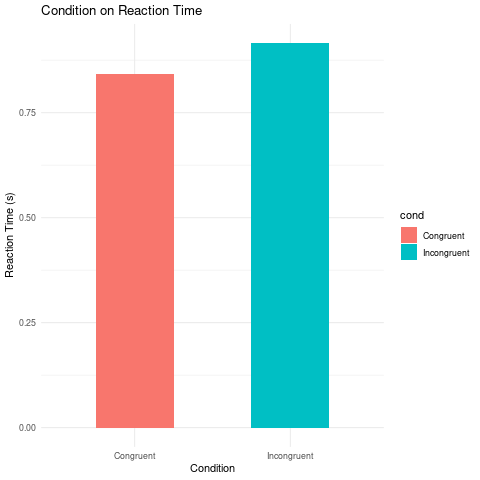
\includegraphics[width=.9\linewidth]{barplot_stroop.png}
\end{center}


\begin{verbatim}
library(ggplot2)

data <- read.csv("/home/keagan/GitRepos/363Stroop/363Stroop_Data_Dec_4.csv")

Lincongruent <- c()
counter = 1
while(counter <= 20) {
  T = data[which(data$Trial == counter & data$Congruent == 0),]
  mean_RT = mean(T$Time)
  Lincongruent = append(Lincongruent, mean_RT)
  counter = counter + 1
}

Lcongruent <- c()
counter = 1
while(counter <= 20) {
  T = data[which(data$Trial == counter & data$Congruent == 1),]
  mean_RT = mean(T$Time)
  Lcongruent = append(Lcongruent, mean_RT)
  counter = counter + 1
}

cond_rt_df <- data.frame(Condition = rep(c("Congruent", "Incongruent"), each = 20), RT = c(Lcongruent, Lincongruent))
df <- data.frame(Congruent = Lcongruent, Incongruent = Lincongruent)
df$Interference <- df$Incongruent - df$Congruent

incongruent_mean <- mean(data[which(data$Congruent == 0),]$Time)
congruent_mean <- mean(data[which(data$Congruent == 1),]$Time)
overall <- data.frame(cond = c("Incongruent", "Congruent"), rt = c(incongruent_mean, congruent_mean))

\end{verbatim}

\begin{center}
\begin{tabular}{lr}
Incongruent & 0.915385980111821\\
Congruent & 0.843044126528736\\
\end{tabular}
\end{center}





\begin{verbatim}

p <- ggplot(overall, aes(x = cond, y = rt, fill = cond)) + geom_bar(stat = "identity", width = 0.5) + labs(title = "Mean Reaction Time", x = "Condition", y = "Reaction Time (s)") + theme_classic() + theme(plot.title = element_text(hjust = 0.5, size = 15, face = "bold"), legend.position = "right", legend.background = element_blank(), legend.box.background = element_rect(colour = "black"), panel.background = element_blank(), panel.grid = element_blank(), panel.border = element_rect(colour = "black", fill = NA, size = 0.75))

p

\end{verbatim}

\begin{center}

\includegraphics[width=.9\linewidth]{converted_stroop2.png}
\end{center}



\begin{verbatim}

density_plot <- ggplot(cond_rt_df, aes(x = RT, color = Condition, fill = Condition)) + geom_density(alpha = 0.5) + labs(title = "Response Time Density Plot", x = "Response Time (s)", y = "Frequency") + theme_classic() + theme(plot.title = element_text(hjust = 0.5, size = 15, face = "bold"), legend.position = "right", legend.background = element_blank(), legend.box.background = element_rect(colour = "black"), panel.background = element_blank(), panel.grid = element_blank(), panel.border = element_rect(colour = "black", fill = NA, size = 0.75)) + xlim(0.25, 1.75)

density_plot

\end{verbatim}

\begin{center}

\includegraphics[width=.9\linewidth]{converted_stroop3.png}
\end{center}



\begin{verbatim}

interference_hist <- ggplot(df, aes(x = Interference)) + geom_histogram(binwidth = 0.05, color = "white", fill = "darkturquoise") + labs(title = "Interference Histogram", x = "Increase in Response Time (s)", y = "Number of Observers") + theme_classic() + theme(plot.title = element_text(hjust = 0.5, size = 15, face = "bold"), panel.background = element_blank(), panel.grid = element_blank(), panel.border = element_rect(colour = "black", fill = NA, size = 0.75))

interference_hist

\end{verbatim}

\begin{center}

\includegraphics[width=.9\linewidth]{converted_stroop4.png}
\end{center}




\begin{verbatim}

RT_congruent <- ggplot(df, aes(x = Congruent)) + geom_histogram(alpha = 0.5, fill = "steelblue") + geom_density(color = "steelblue") + labs(title = "Response Time for Congruent Words", x = "Response Time (s)", y = "Frequency") + theme_classic() + theme(plot.title = element_text(hjust = 0.5, size = 15, face = "bold"), panel.background = element_blank(), panel.grid = element_blank(), panel.border = element_rect(colour = "black", fill = NA, size = 0.75)) + xlim(0.25, 1.75) + ylim(0, 5)

RT_congruent

\end{verbatim}

\begin{center}
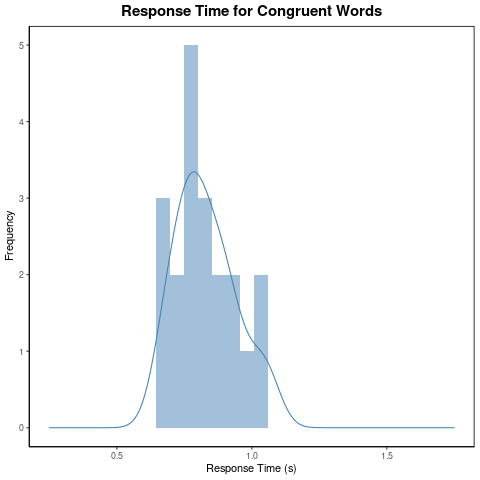
\includegraphics[width=.9\linewidth]{converted_stroop5.png}
\end{center}




\begin{verbatim}

RT_incongruent <- ggplot(df, aes(x = Incongruent)) + geom_histogram(alpha = 0.5, fill = "steelblue") + geom_density(color = "steelblue") + labs(title = "Response Time for Incongruent Words", x = "Response Time (s)", y = "Frequency") + theme_classic() + theme(plot.title = element_text(hjust = 0.5, size = 15, face = "bold"), panel.background = element_blank(), panel.grid = element_blank(), panel.border = element_rect(colour = "black", fill = NA, size = 0.75)) + xlim(0.25, 1.75) + ylim(0, 5)

RT_incongruent

\end{verbatim}

\begin{center}
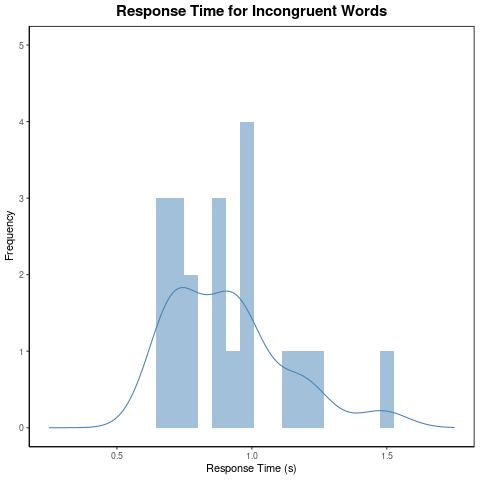
\includegraphics[width=.9\linewidth]{converted_stroop6.png}
\end{center}



\begin{verbatim}

RT_cond <- ggplot(cond_rt_df, aes(x = RT, color = Condition, fill = Condition)) + geom_histogram(color = NA, alpha = 0.5, position = "identity") + geom_density(alpha = 0) + labs(title = "Response Time for Congruent vs. Incongruent Words", x = "Response Time (s)", y = "Frequency") + theme_classic() + theme(plot.title = element_text(hjust = 0.5, size = 15, face = "bold"), legend.position = "right", legend.background = element_blank(), legend.box.background = element_rect(colour = "black"), panel.background = element_blank(), panel.grid = element_blank(), panel.border = element_rect(colour = "black", fill = NA, size = 0.75)) + xlim(0.25, 1.75) + ylim(0, 5)

RT_cond

\end{verbatim}

\begin{center}

\includegraphics[width=.9\linewidth]{converted_stroop7.png}
\end{center}
\end{document}
